\documentclass{article}
\usepackage{graphicx} % Required for inserting images
\usepackage[top=0.9in, bottom=1in, left=1.5in, right=1.5in]{geometry}
\usepackage[utf8]{inputenc}
\usepackage[icelandic]{babel}
\usepackage[T1]{fontenc}
\usepackage[sc]{mathpazo}
\usepackage[parfill]{parskip}
\renewcommand{\baselinestretch}{1.2}
% Tables and lists
\usepackage{booktabs,tabularx}
\usepackage{multirow}
\usepackage{enumerate}
\usepackage{adjustbox}
\usepackage{multicol}
\usepackage{xcolor}
\usepackage{algpseudocode}
\usepackage{algorithm}
\usepackage{tikz}
\usepackage{nicefrac}
\usepackage{changepage}
\usepackage{fancyvrb}
\usepackage{xlop}
\usepackage{hyperref}
\usetikzlibrary{arrows, positioning, calc, graphs}

% Math
\usepackage{amsmath, amsfonts, amssymb, amsthm}
% Graphics

\usepackage{graphicx}
\usepackage{tikz}
% Code environment
\usepackage{minted}
%\usepackage{bm}
%\usepackage{siunitx}
%\usepackage{animate}
%\usepackage{hyperref}
%\usepackage{movie15}
%\usepackage{multicol}
%\usepackage{changepage}
\title{Tölvugrafík Heimadæmi 3}
\author{Ragnar Björn Ingvarsson, rbi3}
\tikzset{->, >=stealth', shorten >=1pt, node distance=2cm,thick, main node/.style={circle,draw,minimum size=3em}}


\begin{document}
\renewcommand\thepage{}
	
	\maketitle

	\newpage
	\setcounter{page}{1}
	\renewcommand\thepage{\arabic{page}}

	\section{}
	\begin{center}
		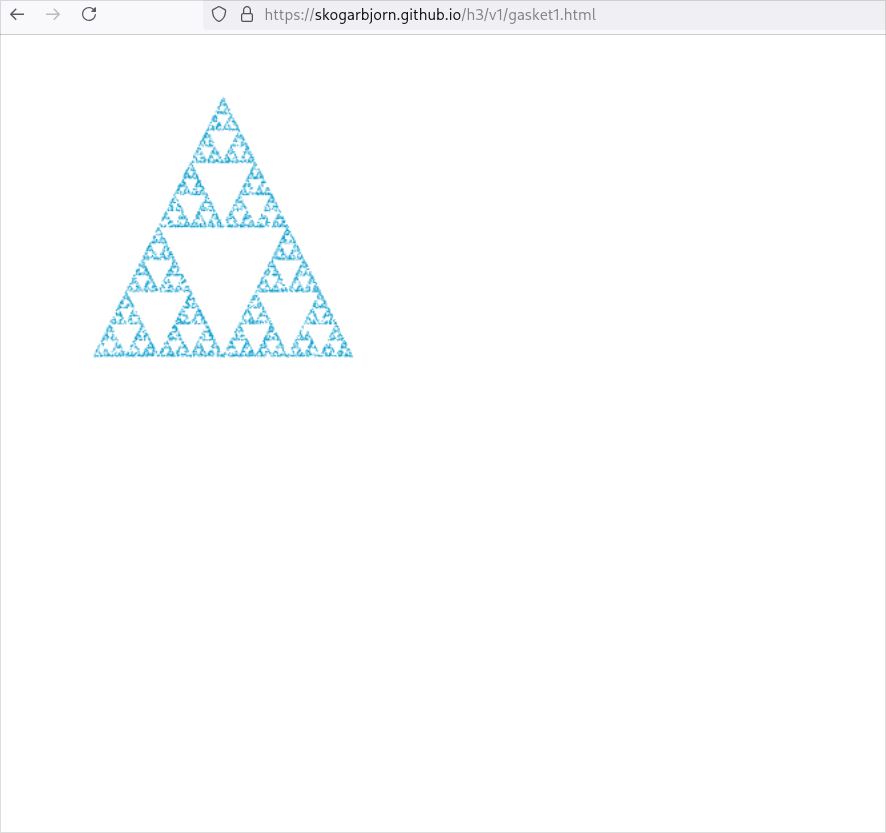
\includegraphics[scale=0.35]{sierpinski.png}
	\end{center}
	\url{https://skogarbjorn.github.io/h3/v1/gasket1.html}

	\section{}
	\begin{center}
		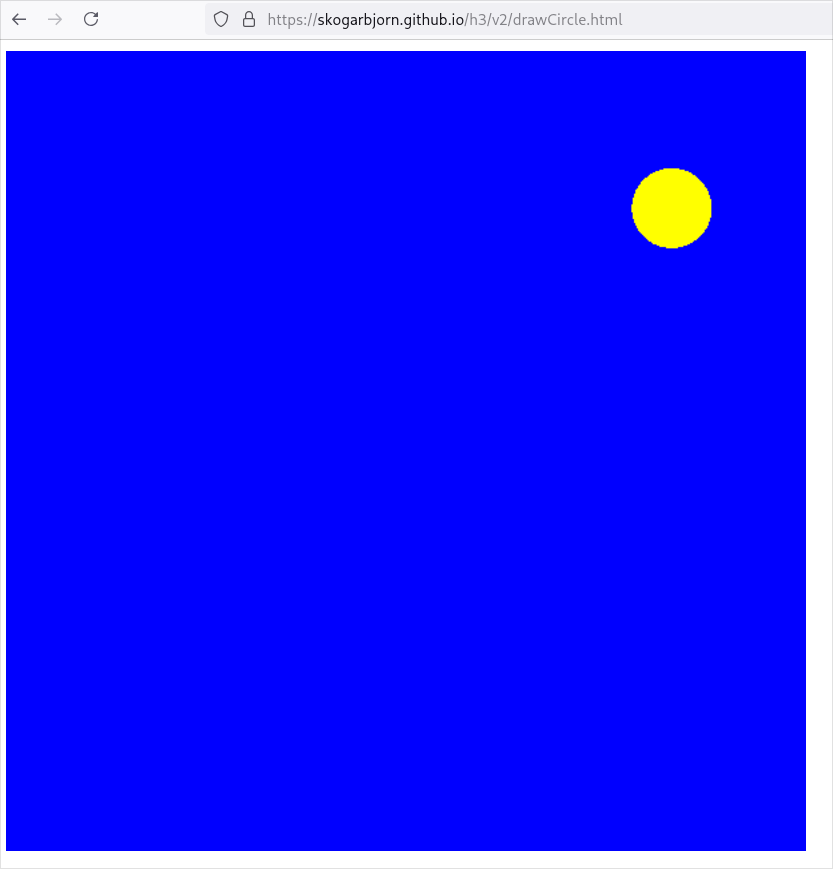
\includegraphics[scale=0.35]{movball.png}
	\end{center}
	\url{https://skogarbjorn.github.io/h3/v2/drawCircle.html}

	\section{}
	\begin{itemize}
		\item[a)] 
			\begin{itemize}
				\item[i)] (2,3)
				\item[ii)] (2,-3)
				\item[iii)] (2,6)
			\end{itemize}
		\item[b)] \textit{a} er 4 þar sem $\frac{4}{-1} = -4$ og \textit{b} 
			er $2$ þar sem $\frac{4}{2}= 2$ og $\frac{-8}{2} = -4$.
	\end{itemize}

	\section{}
	\begin{itemize}
		\item[a)] $u = [2,0]$, $v = [5,0]$ þar sem við fáum innfeldið
				\[\| u\|\| v\| cos\theta\]
				\[=\sqrt{2^2+0^2}\cdot \sqrt{5^2+0^2}\cdot cos(0)\]
				\[=2\cdot5\cdot1\]
				\[=10\]
		\item[b)] $u = [2,0]$, $v = [-5,0]$ þar sem við fáum innfeldið
				\[\|u\|\|v\|cos\theta\]
				\[=\sqrt{2^2+0^2}\cdot\sqrt{(-5)^2+0^2}\cdot cos(180)\]
				\[=2\cdot5\cdot -1\]
				\[=-10\]
		\item[c)] Við sjáum þá að
			\[(s\textbf{u})\cdot\textbf{v}\]
			\[= [su_n, su_{n-1}, ...,su_0]\cdot\textbf{v}\]
			\[=\sqrt{(su_n)^2 + (su_{n-1})^2 + ...+ (su_0)^2}\sqrt{v_m^2 + 
			v_{m-1}^2 + ... + v_0^2}\cdot cos\theta\]
			\[=\sqrt{s^2u_n^2 + s^2u_{n-1}^2 + ... + s^2u_0^2}\sqrt{v_m^2 + 
			v_{m-1}^2 + ... + v_0^2}\cdot cos\theta\]
			\[=\sqrt{s^2(u_n^2 + u_{n-1}^2 + ... + s_0^2)}\sqrt{v_m^2 + 
			v_{m-1}^2 + ... + v_0^2}\cdot cos\theta\]
			\[=s\sqrt{u_n^2 + u_{n-1}^2 + ... + s_0^2}\sqrt{v_m^2 + 
			v_{m-1}^2 + ... + v_0^2}\cdot cos\theta\]
			\[=s\|\textbf{u}\|\|\textbf{v}\|cos\theta\]
			\[=s(\|\textbf{u}\|\|\textbf{v}\|cos\theta)\]
			\[=s(\textbf{u}\cdot\textbf{v})\]
	\end{itemize}

	\section{}

	\begin{algorithm}
	\caption{Athugar hvort $n$ punktar liggi í sömu sléttu}
	\begin{algorithmic}
		\Require $n>3$ \Comment{$points$ er af lengd $n$}
		\State $a \gets points_0$
		\State $b \gets points_1$
		\State $c \gets points_2$
		\State $ab \gets b-a$
		\State $ac \gets c-a$
		\State $V \gets ab \times ac$ \Comment{$\times$ er cross product}
		\While{$i\gets3$ is less than $n$}
			\State $ad \gets points_i-a$
			\If{$ad\cdot V \neq 0$} \Comment{$\cdot$ er dot product}
				\State\Return false
			\EndIf
		\EndWhile
		\State\Return true
	\end{algorithmic}
	\end{algorithm}

\end{document}
